\clearpage
\section{\texorpdfstring{\underline{Graph Algorithms}}{Graph Algorithms}}
\subsection{Graph Representations}
\subsubsection{Graph Transpose}
\textbf{Problem Type:} Computing transpose $G^T$ of a directed graph $G=(V,E)$

\textbf{What to Look For:}
\begin{itemize}[noitemsep,leftmargin=*]
    \item Graph representation type (matrix/list)
    \item Direction of edges must be reversed
    \item Time complexity analysis required
\end{itemize}

\textbf{Key Definitions:}
\begin{itemize}[noitemsep,leftmargin=*]
    \item $G^T = (V,E^T)$ where $E^T = \{(v,u) \mid (u,v) \in E\}$
    \item $|V| = n$ (number of vertices)
    \item $|E|$ (number of edges)
\end{itemize}

\textbf{Solution for Adjacency Matrix:}
\begin{enumerate}[leftmargin=*,noitemsep]
    \item Given matrix $M_G$, create $M_G^T$ by swapping entries:
    \[ M = \begin{pmatrix}
        m_{11} & m_{12} & \cdots & m_{1n}\\
        m_{21} & m_{22} & \cdots & m_{2n}\\
        \vdots & \vdots & \ddots & \vdots\\
        m_{n1} & m_{n2} & \cdots & m_{nn}
    \end{pmatrix} \]
    
    \[ M^T = \begin{pmatrix}
        m_{11} & m_{21} & \cdots & m_{n1}\\
        m_{12} & m_{22} & \cdots & m_{n2}\\
        \vdots & \vdots & \ddots & \vdots\\
        m_{1n} & m_{2n} & \cdots & m_{nn}
    \end{pmatrix} \]

    \item Example:
    \[ M = \begin{pmatrix}1 & 2\\ 3 & 4\end{pmatrix}, 
       M^T = \begin{pmatrix}1 & 3\\ 2 & 4\end{pmatrix} \]
    
    \item Time Complexity: $\Theta(n^2)$
        \begin{itemize}[noitemsep]
            \item Must swap $n^2-n$ entries (excluding diagonal)
            \item Each swap is $O(1)$
        \end{itemize}
\end{enumerate}

\textbf{Solution for Adjacency List:}
\begin{enumerate}[leftmargin=*,noitemsep]
    \item Create empty adjacency lists for $G^T$: $O(n)$
    \item For each vertex $v$ in $G$:
        \begin{itemize}[noitemsep]
            \item For each edge $(v,w)$ in $v$'s adjacency list
            \item Add $v$ to $w$'s list in $G^T$
        \end{itemize}
    \item Time Complexity: $\Theta(|V| + |E|)$
        \begin{itemize}[noitemsep]
            \item Creating lists: $O(|V|)$
            \item Processing edges: $O(|E|)$
        \end{itemize}
\end{enumerate}

\textbf{Comparison:}
\begin{itemize}[noitemsep,leftmargin=*]
    \item Matrix: $\Theta(n^2)$ always
    \item List: $\Theta(|V| + |E|)$ which is better for sparse graphs
    \item List requires more complex implementation
\end{itemize}

\textbf{Common Mistakes to Avoid:}
\begin{itemize}[noitemsep,leftmargin=*]
    \item Don't forget self-loops (diagonal elements)
    \item Don't count diagonal elements in matrix swaps
    \item Remember to initialize all new lists in adjacency list solution
    \item Don't confuse $|V|$ and $|E|$ in complexity analysis
\end{itemize}

\FloatBarrier

\subsection{Shortest Paths}
\subsubsection{Dijkstra's Algorithm Limitations}
\textbf{Problem Type:} Counterexample for Dijkstra with negative weights

\textbf{What to Look For:}
\begin{itemize}[noitemsep,leftmargin=*]
    \item Directed graph with negative weights
    \item Minimal example showing algorithm failure
    \item Negative cycle demonstration
\end{itemize}

\textbf{Solution:}
\begin{enumerate}[leftmargin=*,noitemsep]
    \item Consider this directed graph:
    \begin{center}
    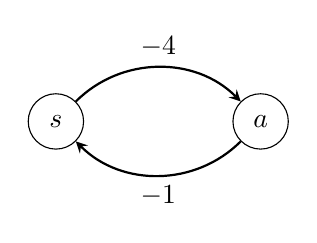
\begin{tikzpicture}[
        scale=1.3,
        vertex/.style={circle,draw,minimum size=20pt,inner sep=0pt}
    ]
        % Vertices
        \node[vertex] (s) at (0,0) {$s$};
        \node[vertex] (a) at (2,0) {$a$};
        
        % Curved edges
        \draw[thick,->,>=stealth] (s) to[bend left=45] node[above] {$-4$} (a);
        \draw[thick,->,>=stealth] (a) to[bend left=45] node[below] {$-1$} (s);
    \end{tikzpicture}
    \end{center}

    \item Why Dijkstra fails:
    \begin{itemize}[noitemsep]
        \item Initial distance to $a$: $-4$
        \item After one cycle: $-5$
        \item After two cycles: $-6$
        \item Continues to decrease indefinitely
    \end{itemize}
\end{enumerate}

\textbf{Key Properties:}
\begin{itemize}[noitemsep,leftmargin=*]
    \item Any negative cycle causes Dijkstra to fail
    \item Algorithm assumes:
        \begin{itemize}[noitemsep]
            \item Edge weights are non-negative
            \item Shortest paths exist (no negative cycles)
        \end{itemize}
    \item For negative weights, use Bellman-Ford instead
\end{itemize}

\textbf{Common Mistakes to Avoid:}
\begin{itemize}[noitemsep,leftmargin=*]
    \item Single negative edge isn't enough
    \item Example must have negative total cycle weight
\end{itemize}

\FloatBarrier
